\chapter{Methods}
\label{chapter:methods}
This chapter discusses the design of the study. First, research questions are introduced.
Second, research hypothesis is made based on the reviewed practices \& related research findings introduced in the chapter \ref{chapter:background}
and features of studied testing frameworks explained in chapter \ref{chapter:environment}.
Third, the empirical study and its methodology are explained in detail. Finally, limitations to the study methods are discussed.

\section{Research questions}
This thesis studies low level testing done with xUnit family testing framework JUnit and how it changes after putting
an implementation level BDD testing framework into operation. The scope in research is testing Java-code. The following
research questions are aimed to highlight the change in low level testing after the testing framework change:
\begin{enumerate}
\item \textbf{RQ1}: How does behavior driven testing frameworks change developer practices working with automated low level testing compared to JUnit framework?
\item \textbf{RQ2}: How does behavior driven testing frameworks change developer perception of working with automated low level testing compared to JUnit framework?
\item \textbf{RQ3}: How does behavior driven testing frameworks change written low level test cases and test code coverage compared to JUnit framework?
\end{enumerate}

\section{Research hypothesis} %1p
    The following hypothesis statements are derived from the mentioned benefits of BDD literature in chapter \ref{chapter:background} and features of BDD
    testing frameworks illustrated in previous chapter. These statements adhere directly to common problems found in unit
    testing practitioner research mentioned in section \ref{section:research} in chapter \ref{chapter:background}.
    \begin{addmargin}[0em]{0em}
    \vspace{10px}
    \textbf{Statement 1:} Developers will write more granular test cases
    \vspace{5px}
    \newline
    As has been noted before in benefits of implementation level behavior driven development, BDD testing frameworks operating on this
    level aim to produce granular test cases with descriptive named test methods~\cite{chelimsky2010rspec}~\cite{astels2006new}.
    For example RSpec was originally intended to help the shifting of viewpoint from 1-1 relationship between test-code
    and only one test method per function to more granular test cases~\cite{astels2006new}.
    Compared to earlier average in the project, statement should be visible in test cases through more measured test methods
    per method of component under test. In addition, the phenomena is also studied with a participant survey.
    \end{addmargin}

    \begin{addmargin}[0em]{0em}
    \vspace{10px}
    \textbf{Statement 2:} Developers will find it easier to understand test cases
    \vspace{5px}
    \newline
    As stated earlier, implementation level BDD testing frameworks should produce test cases of the component under test,
    that \textbf{describe behavior} with examples~\cite{chelimsky2010rspec}~\cite{astels2006new}~\cite{amodeo2015learning}.
    The close to natural language DSL used to create these behavior specifying tests with BDD testing frameworks should
    have a natural tendency to "force" developers to write more descriptive tests. This is provided for example
    with xSpec family keywords \textit{describe} \& \textit{it} and with Gherkin family \textit{Given, When \& Then}-steps.
    The context, stimulus and assertions of the tests should be more visible with these mentioned structures and the test output
    should be more understandable~\cite{smart2014bdd}. Statement is measured with a survey and interview.
    \end{addmargin}

    \begin{addmargin}[0em]{0em}
    \vspace{10px}
    \textbf{Statement 3:} Developers will find it easier to maintain code
    \vspace{5px}
    \newline
    Implementation level BDD specifications should produce up-to-date living documentation, which can help in overall
    maintenance of the the system~\cite{smart2014bdd}. Especially the maintaining of test cases should be easier
    with repetition reducing techniques provided by these BDD testing frameworks~\cite{chelimsky2010rspec}~\cite{kapelonis2016java}.
    xSpec family nested group examples and lifecycle hooks should allow efficient repetition removal compared to traditional xUnit family testing frameworks.
    Data Driven Testing DSL of Spock testing framework should allow to more easily test parameter variations and remove
    the need for separate test methods, therefore making it easier to maintain the test case.
    Statement is measured with a survey and interview.
    \end{addmargin}

    \begin{addmargin}[0em]{0em}
    \vspace{10px}
    \textbf{Statement 4:} Developers will perceive working with low level automated testing more enjoyable.
    \vspace{5px}
    \newline
    This statement is a combination of the three earlier statements. By changing the used practices and language in low level testing,
    the overall result should appear as more enjoyable low level testing for developers. Especially the statements 2 and 3, easier understanding
    and maintaining of test cases should affect how automated low level testing is perceived.
    Statement is measured with a survey and interview.
    \end{addmargin}

\section{Empirical study}
First in this section the type of study is determined, together with rationale and objectives of it. Second, the case selection
is explained with process for selecting teams and developers. Third, the data selection methods of this empirical study are
explained. Finally, threats to validity and limitations in this study are reviewed.

\subsection{Type of study and purpose}
    This section explains the design of the empirical \textbf{case study} collecting evidence from multiple sources with methodological triangulation.
    The data was collected from multiple projects and participants with surveys and interviews.
    Case study data collecting was enriched with observations from
    multiple projects and their test code changes. Survey data can be categorized as quantative, interview data as qualitative and observation data as quantative.
    This study follows the pattern of deductive research, starting with background \textit{theory} and \textit{hypothesis} followed by
    \textit{observations} and \textit{confirmation}. This is visible through combined practices
    from experimental research with identified problems and predicted answer to found problems in the form of hypothesis.
    Case study methodology was build with suggested best practices for empirical research in software engineering~\cite{kitchenham2002preliminary} and case
    study research~\cite{runeson2012case}.

    \textbf{Rationale} of this case study was to improve existing traditional low level automated testing practices research with studying
    relevant technologies used in the industry. At the same time, this case study could act as a starting point for future
    research on the differences of traditional xUnit testing frameworks and implementation level BDD testing frameworks for larger
    scale studies.

    \textbf{Objective} of the study was to compare traditional xUnit testing frameworks and implementation level BDD testing frameworks
    and how they change the developer practices and perception towards low level automated testing. The change was also measured
    with changes in written test code.
    As this thesis is done at industry context, the purpose was also to determine how well these
    new testing frameworks in JVM context could work for future use in Java projects in the studied company.


\subsection{Process for selecting teams and developers}
    The study was conducted in industry context at IT-consulting software firm \textbf{Vincit Plc}, Helsinki Mikonkatu 15 office.
    Related to objective of studying the automated low level testing differences, context for the development environment was chosen as JVM.
    JVM provides interesting possibilities through various programming languages in use for low level automated testing.
    For the selection of teams, there was limitations; team should be implementing a Java-based Spring Framework project with prior JUnit
    unit and integration testing in place. Limiting factor in team selection was also the amount of effort available,
    as my intention was to graduate in the current spring semester of 2017.  This filtered out projects that could not start
    the study before April.

    With these constraints, two projects and their teams were chosen to be studied. The teams were first introduced to
    implementation level BDD testing frameworks and two months after the initial introduction and time in use for these BDD
    frameworks, the data collecting was ended. The two months time was chosen to see, how the early adoption of new technologies had gone.
    The limited time available was also a practical constraint that resulted to study only for two months time. All the participants
    in this study were restricted to developers, as the purpose was to study developer testing practices. The projects
    A and B, and how developers chose which BDD testing framework to take into use, are explained in more detail in the next chapter.


\subsection{Data collection}
    Selection of data included filtering of participants in the project. Participants were filtered to backend developers
    whom were developing with the Java Spring Framework and thus using JUnit for low level testing purposes.

    Data collection from projects is done with methodological triangulation using first degree study participant interviews, second degree
    participant surveys and third degree quantative test code analysis. The main tool is the second degree surveys.
    First the \textbf{interview for demographic purposes} is explained. Second, the two \textbf{surveys} used to answer
    \textbf{RQ1 and RQ2} are examined. In addition to surveys for RQ1 and RQ2, an \textbf{interview} was conducted at the end with participants to
    learn more about general thoughts on the new testing frameworks used.
    Third, \textbf{test code analysis}, aimed to help answering \textbf{RQ3}, is defined.

    \subsubsection{Interview for demographic purposes}
    Participant demographics were studied with recorded semi-structured interviews~\cite{cohen2006qualitative}.
    The interview was constructed following the guidelines of suggested best practices~\cite{kitchenham2002preliminary}.
    The results of interviews and the analyzed demographics are shown in the chapter
    \ref{chapter:results}. The questions of the interview can be found from Appendix \ref{chapter:interview} section
    \ref{section:demographic}.

    \subsubsection{Survey about low level automated testing with JUnit}
    An online survey was build to answer research questions RQ1 and RQ2, the changes in low level testing practices and perception.
    The survey was designed and built using \textit{LimeSurvey}~\cite{limesurvey}. The reason to use survey as the main tool for data collection
    was the related unit testing research surveys~\cite{runeson2006survey}~\cite{williams2009effectiveness}~\cite{daka2014survey}~\cite{li2016automatically}.
    Some of the survey questions were interesting starting points
    for the built survey in this study. As there were many survey questions, it was logical to conduct the identifying
    of the baseline for low level testing practices and perception with a survey. Additional motivation to use
    survey was to quantify results and to provide a more specific survey question set to study problematic
    areas risen from related research problems.
    % TODO: here some text how results were extracted and further analyzed

    Copied survey questions were used as close to their original form as possible.
    The question scales were unchanged, ranging from 1 to 5 and 1 to 7 point \textbf{Likert scale} questions
    to one summing percentage question. The changed part was some of the words in few questions.
    Changed words were from \textit{"unit"} to \textit{"low level"},
    resulting in questions that take into consideration both unit and integration level testing.

    Questions created for this research were mainly 1 to 7 point Likert scale questions.
    The reason to use 7 point Likert scale was to increase the discriminating power of the questions~\cite{cummins2000we}.
    At the end of the survey \textbf{Network Promoter Score (NPS)}~\cite{reichheld2003one} was used to see how enthuastic and "loyal" the participants
    were at the beginning of the study to low level automated testing in general and in more specific to JUnit.
    The implementation of survey, its questions and how it relates to related research survey questions can be found from Appendix...
    %-Existing base questions explained with references to original publications\newline
    %-NPS explained\newline
    %-Implementation of JUnit survey / screenshots / questions shown\newline
    \subsubsection{Survey about changes in low level automated testing after introduction of BDD testing frameworks}
    The second survey used all the questions (with modifications) from the first survey regarding JUnit testing practices and
    also added couple additional questions related to selected BDD testing framework. The survey was built using LimeSurvey.
    Modifications to questions include changing the question setup to a direct comparison to JUnit.
    For example, in case of a original 5 point scale Likert question
    \begin{figure}[H]
      \begin{center}
        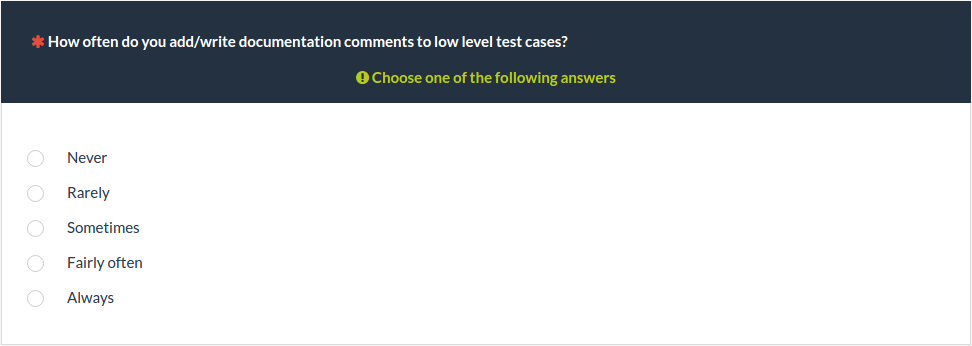
\includegraphics[width=13.7cm]{images/survey-org-comments.png}
        \caption{JUnit survey 5 point scale Likert question}
        \label{fig:survey-junit-comments}
      \end{center}
    \end{figure}
    \begin{addmargin}[0em]{0em}
    The resulting comparison question looks following
    \end{addmargin}
    \begin{figure}[H]
      \begin{center}
        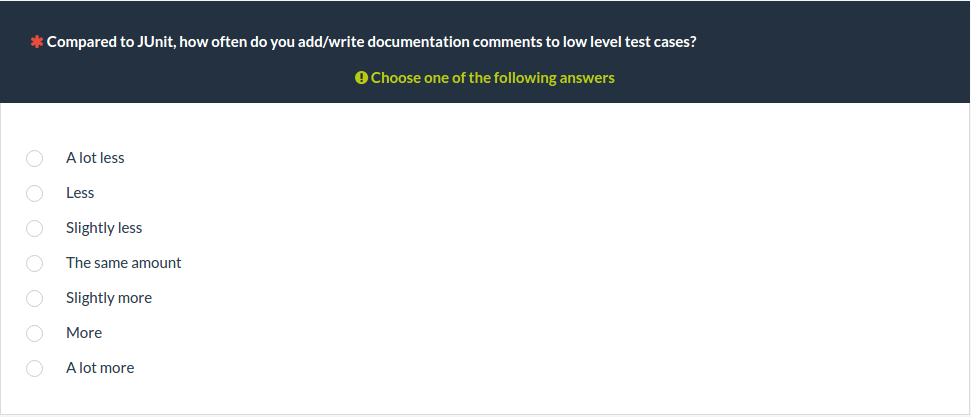
\includegraphics[width=13.7cm]{images/survey-bdd-comments.png}
        \caption{Spectrum survey 7 point scale Likert comparison question}
        \label{fig:survey-bdd-comments}
      \end{center}
    \end{figure}

    The reason to change the questions was to provide direct comparison between the test frameworks.
    If the same question set was repeated to gather insight on the new BDD testing framework, there exists the risk that
    the participant doesn't remember what he or she answered the last time. It could result in choosing the same answer option,
    despite the slight change in practice or perception in testing.

    The used question types were mostly 1 to 7 point Likert scale questions for the direct comparisons, combined with a few NPS questions for
    determining developer loyalty towards low level automated testing in general and also towards the new BDD testing framework.
    Couple additional free text questions were also added.
    The implementation of survey, its questions and how it relates to related research survey questions can be found from Appendix...
    %-Implementation of Spock/Spectrum survey / screenshots / questions shown\newline\newline

    \subsubsection{Interview about benefits and drawbacks of new BDD testing framework}

    \subsubsection{Test code analysis}
    -Mine repositories test code\newline
        -Define all software measures fully, including the entity, attribute, unit and counting rules.

\section{Threats to validity}
-Response bias\newline
-Presence of a "champion" in influencing the use & first impressions\newline
-Threats to validity of questionnaire\newline\newline
\section{Limitations of the case study}
-limited time\newline
-limited number of participants\newline
-limited amount of new test cases\newline


